\documentclass[aspectratio=169]{beamer}

% Minimal theme
\usetheme{default}
\usecolortheme{dove}

% Remove navigation symbols
\setbeamertemplate{navigation symbols}{}
\setbeamertemplate{footline}{%
  \hfill{\large\insertframenumber\,/\,\inserttotalframenumber}\hspace{0.8em}\vspace{0.5em}%
}

% Colors
\definecolor{popblue}{RGB}{52, 101, 164}
\definecolor{sampred}{RGB}{204, 0, 0}
\definecolor{paramgreen}{RGB}{0, 140, 70}
\definecolor{lightbg}{RGB}{245, 245, 250}
\definecolor{warnred}{RGB}{180, 40, 40}
\definecolor{orange1}{RGB}{220, 120, 0}
\definecolor{violet1}{RGB}{120, 50, 160}

\setbeamercolor{frametitle}{fg=popblue}
\setbeamercolor{title}{fg=popblue}

% Packages
\usepackage{pgfplots}
\usepackage{tikz}
\usetikzlibrary{shapes, arrows.meta, positioning, calc, decorations.pathreplacing}
\pgfplotsset{compat=1.18}
\usepackage{amsmath, amssymb}
\usepackage{array}
\usepackage[T1]{fontenc}

\title{Emergence}
\subtitle{Phase Transitions $\cdot$ Emergent Abilities $\cdot$ The Mirage Debate $\cdot$ Grokking}
\date{}

\begin{document}

% ============================================================
% TITLE
% ============================================================
\begin{frame}
\titlepage
\end{frame}

% ============================================================
% WHAT IS EMERGENCE?
% ============================================================
\begin{frame}
\frametitle{What is emergence?}

\begin{center}
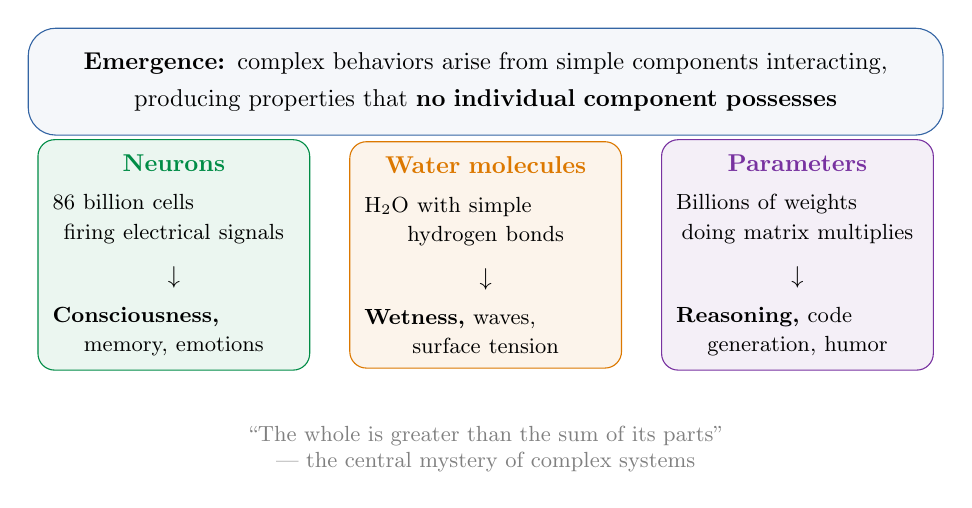
\begin{tikzpicture}[scale=0.88, transform shape]
  % Definition
  \node[draw=popblue, fill=popblue!5, rounded corners=10pt, text width=12.5cm, align=center, inner sep=10pt, font=\normalsize] at (0, 3) {
    \textbf{Emergence:} complex behaviors arise from simple components interacting,\par\vspace{3pt}
    producing properties that \textbf{no individual component possesses}
  };

  % Three examples in a row
  \node[draw=paramgreen, fill=paramgreen!8, rounded corners=6pt, text width=3.5cm, align=center, inner sep=6pt] at (-4.5, 0.5) {
    \textbf{\textcolor{paramgreen}{Neurons}}\par\vspace{4pt}
    {\small 86 billion cells\newline firing electrical signals}\par\vspace{6pt}
    $\downarrow$\par\vspace{4pt}
    {\small\textbf{Consciousness,}\newline memory, emotions}
  };

  \node[draw=orange1, fill=orange1!8, rounded corners=6pt, text width=3.5cm, align=center, inner sep=6pt] at (0, 0.5) {
    \textbf{\textcolor{orange1}{Water molecules}}\par\vspace{4pt}
    {\small H$_2$O with simple\newline hydrogen bonds}\par\vspace{6pt}
    $\downarrow$\par\vspace{4pt}
    {\small\textbf{Wetness,} waves,\newline surface tension}
  };

  \node[draw=violet1, fill=violet1!8, rounded corners=6pt, text width=3.5cm, align=center, inner sep=6pt] at (4.5, 0.5) {
    \textbf{\textcolor{violet1}{Parameters}}\par\vspace{4pt}
    {\small Billions of weights\newline doing matrix multiplies}\par\vspace{6pt}
    $\downarrow$\par\vspace{4pt}
    {\small\textbf{Reasoning,} code\newline generation, humor}
  };

  % Bottom
  \node[font=\small, text=gray, text width=12cm, align=center] at (0, -2.3) {
    ``The whole is greater than the sum of its parts'' --- the central mystery of complex systems
  };
\end{tikzpicture}
\end{center}
\end{frame}

% ============================================================
% ANT COLONIES
% ============================================================
\begin{frame}
\frametitle{Emergence in nature: ant colonies}
\vspace{-0.3cm}
\begin{center}
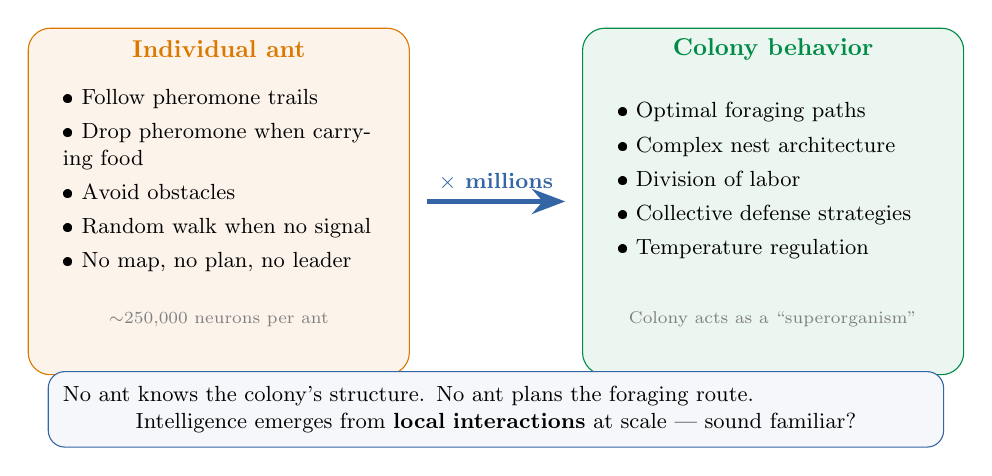
\begin{tikzpicture}[scale=0.88, transform shape]
  % Individual ant rules (left)
  \node[draw=orange1, fill=orange1!8, rounded corners=8pt, minimum width=5.5cm, minimum height=5cm] at (-4, 0.5) {};
  \node[font=\normalsize\bfseries, text=orange1] at (-4, 2.7) {Individual ant};

  \node[font=\small, text width=4.5cm, align=left] at (-4, 0.8) {
    \textbullet\ Follow pheromone trails\par\vspace{3pt}
    \textbullet\ Drop pheromone when carrying food\par\vspace{3pt}
    \textbullet\ Avoid obstacles\par\vspace{3pt}
    \textbullet\ Random walk when no signal\par\vspace{3pt}
    \textbullet\ No map, no plan, no leader
  };
  \node[font=\scriptsize, text=gray] at (-4, -1.2) {$\sim$250,000 neurons per ant};

  % Arrow
  \draw[-Stealth, very thick, popblue, line width=2pt] (-1, 0.5) -- (1, 0.5)
    node[midway, above, font=\small\bfseries, text=popblue] {$\times$ millions};

  % Colony-level behavior (right)
  \node[draw=paramgreen, fill=paramgreen!8, rounded corners=8pt, minimum width=5.5cm, minimum height=5cm] at (4, 0.5) {};
  \node[font=\normalsize\bfseries, text=paramgreen] at (4, 2.7) {Colony behavior};

  \node[font=\small, text width=4.5cm, align=left] at (4, 0.8) {
    \textbullet\ Optimal foraging paths\par\vspace{3pt}
    \textbullet\ Complex nest architecture\par\vspace{3pt}
    \textbullet\ Division of labor\par\vspace{3pt}
    \textbullet\ Collective defense strategies\par\vspace{3pt}
    \textbullet\ Temperature regulation
  };
  \node[font=\scriptsize, text=gray] at (4, -1.2) {Colony acts as a ``superorganism''};

  % Bottom insight
  \node[draw=popblue, fill=popblue!5, rounded corners=6pt, text width=12.5cm, align=center, inner sep=6pt, font=\small] at (0, -2.5) {
    No ant knows the colony's structure. No ant plans the foraging route.\newline
    Intelligence emerges from \textbf{local interactions} at scale --- sound familiar?
  };
\end{tikzpicture}
\end{center}
\end{frame}

% ============================================================
% CELLS TO ORGANS
% ============================================================
\begin{frame}
\frametitle{Emergence in nature: cells to organs}
\vspace{-0.3cm}
\begin{center}
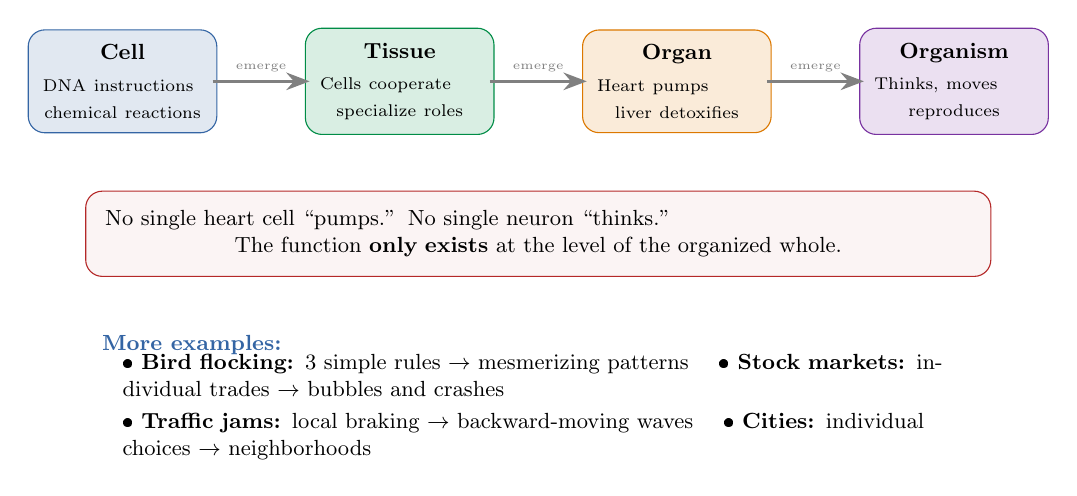
\begin{tikzpicture}[scale=0.88, transform shape]
  % Hierarchy
  \node[draw=popblue, fill=popblue!15, rounded corners=6pt, text width=2.3cm, font=\small, inner sep=6pt, align=center] at (-5.5, 2) {
    \textbf{Cell}\par\vspace{2pt}
    {\scriptsize DNA instructions\newline chemical reactions}
  };

  \node[draw=paramgreen, fill=paramgreen!15, rounded corners=6pt, text width=2.3cm, font=\small, inner sep=6pt, align=center] at (-1.5, 2) {
    \textbf{Tissue}\par\vspace{2pt}
    {\scriptsize Cells cooperate\newline specialize roles}
  };

  \node[draw=orange1, fill=orange1!15, rounded corners=6pt, text width=2.3cm, font=\small, inner sep=6pt, align=center] at (2.5, 2) {
    \textbf{Organ}\par\vspace{2pt}
    {\scriptsize Heart pumps\newline liver detoxifies}
  };

  \node[draw=violet1, fill=violet1!15, rounded corners=6pt, text width=2.3cm, font=\small, inner sep=6pt, align=center] at (6.5, 2) {
    \textbf{Organism}\par\vspace{2pt}
    {\scriptsize Thinks, moves\newline reproduces}
  };

  \draw[-Stealth, very thick, gray] (-4.2, 2) -- (-2.8, 2) node[midway, above, font=\tiny] {emerge};
  \draw[-Stealth, very thick, gray] (-0.2, 2) -- (1.2, 2) node[midway, above, font=\tiny] {emerge};
  \draw[-Stealth, very thick, gray] (3.8, 2) -- (5.2, 2) node[midway, above, font=\tiny] {emerge};

  % Key point
  \node[draw=warnred, fill=warnred!5, rounded corners=6pt, text width=12.5cm, align=center, inner sep=8pt, font=\small] at (0.5, -0.2) {
    No single heart cell ``pumps.'' No single neuron ``thinks.''\newline
    The function \textbf{only exists} at the level of the organized whole.
  };

  % More examples
  \node[font=\small\bfseries, text=popblue] at (-4.5, -1.8) {More examples:};
  \node[font=\small, text width=12cm, align=left] at (0.5, -2.7) {
    \textbullet~\textbf{Bird flocking:} 3 simple rules $\to$ mesmerizing patterns
    \quad \textbullet~\textbf{Stock markets:} individual trades $\to$ bubbles and crashes\par\vspace{2pt}
    \textbullet~\textbf{Traffic jams:} local braking $\to$ backward-moving waves
    \quad \textbullet~\textbf{Cities:} individual choices $\to$ neighborhoods
  };
\end{tikzpicture}
\end{center}
\end{frame}

% ============================================================
% PHASE TRANSITIONS
% ============================================================
\begin{frame}
\frametitle{Phase transitions: emergence in physics}
\vspace{-0.4cm}
\begin{center}
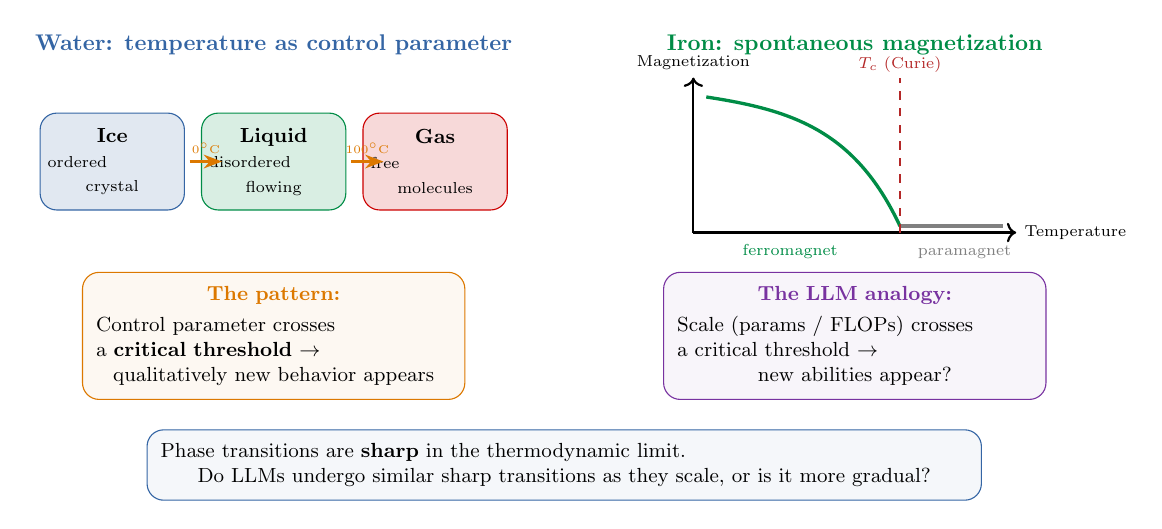
\begin{tikzpicture}[scale=0.82, transform shape]
  % Water example
  \node[font=\normalsize\bfseries, text=popblue] at (-4.5, 3.3) {Water: temperature as control parameter};

  % Three phases
  \node[draw=popblue, fill=popblue!15, rounded corners=6pt, text width=2cm, minimum height=1.5cm, font=\small, align=center] at (-7, 1.5) {\textbf{Ice}\par{\scriptsize ordered\newline crystal}};

  \node[draw=paramgreen, fill=paramgreen!15, rounded corners=6pt, text width=2cm, minimum height=1.5cm, font=\small, align=center] at (-4.5, 1.5) {\textbf{Liquid}\par{\scriptsize disordered\newline flowing}};

  \node[draw=sampred, fill=sampred!15, rounded corners=6pt, text width=2cm, minimum height=1.5cm, font=\small, align=center] at (-2, 1.5) {\textbf{Gas}\par{\scriptsize free\newline molecules}};

  \draw[-Stealth, thick, orange1] (-5.8, 1.5) -- (-5.3, 1.5) node[midway, above, font=\tiny] {0$^\circ$C};
  \draw[-Stealth, thick, orange1] (-3.3, 1.5) -- (-2.8, 1.5) node[midway, above, font=\tiny] {100$^\circ$C};

  % Ferromagnet example
  \node[font=\normalsize\bfseries, text=paramgreen] at (4.5, 3.3) {Iron: spontaneous magnetization};

  % Temperature vs magnetization sketch
  \draw[thick, ->] (2, 0.4) -- (7, 0.4) node[right, font=\scriptsize] {Temperature};
  \draw[thick, ->] (2, 0.4) -- (2, 2.8) node[above, font=\scriptsize] {Magnetization};

  % Curve: high magnetization below Tc, drops to zero at Tc
  \draw[very thick, paramgreen] (2.2, 2.5) .. controls (3.5, 2.3) and (4.5, 2) .. (5.2, 0.5);
  \draw[very thick, gray] (5.2, 0.5) -- (6.8, 0.5);

  % Tc annotation
  \draw[dashed, warnred] (5.2, 0.4) -- (5.2, 2.8);
  \node[font=\scriptsize, text=warnred] at (5.2, 3) {$T_c$ (Curie)};

  \node[font=\scriptsize, text=paramgreen] at (3.5, 0.1) {ferromagnet};
  \node[font=\scriptsize, text=gray] at (6.2, 0.1) {paramagnet};

  % The analogy
  \node[draw=orange1, fill=orange1!5, rounded corners=6pt, text width=5.5cm, align=center, inner sep=6pt, font=\small] at (-4.5, -1.2) {
    \textbf{\textcolor{orange1}{The pattern:}}\par\vspace{3pt}
    Control parameter crosses\newline a \textbf{critical threshold} $\to$\newline qualitatively new behavior appears
  };

  \node[draw=violet1, fill=violet1!5, rounded corners=6pt, text width=5.5cm, align=center, inner sep=6pt, font=\small] at (4.5, -1.2) {
    \textbf{\textcolor{violet1}{The LLM analogy:}}\par\vspace{3pt}
    Scale (params / FLOPs) crosses\newline a critical threshold $\to$\newline new abilities appear?
  };

  % Bottom
  \node[draw=popblue, fill=popblue!5, rounded corners=6pt, text width=12.5cm, align=center, inner sep=6pt, font=\small] at (0, -3.2) {
    Phase transitions are \textbf{sharp} in the thermodynamic limit. \newline
    Do LLMs undergo similar sharp transitions as they scale, or is it more gradual?
  };
\end{tikzpicture}
\end{center}
\end{frame}

% ============================================================
% EMERGENT ABILITIES IN LLMS
% ============================================================
\begin{frame}
\frametitle{Emergent abilities in LLMs}
\vspace{-0.3cm}
\begin{center}
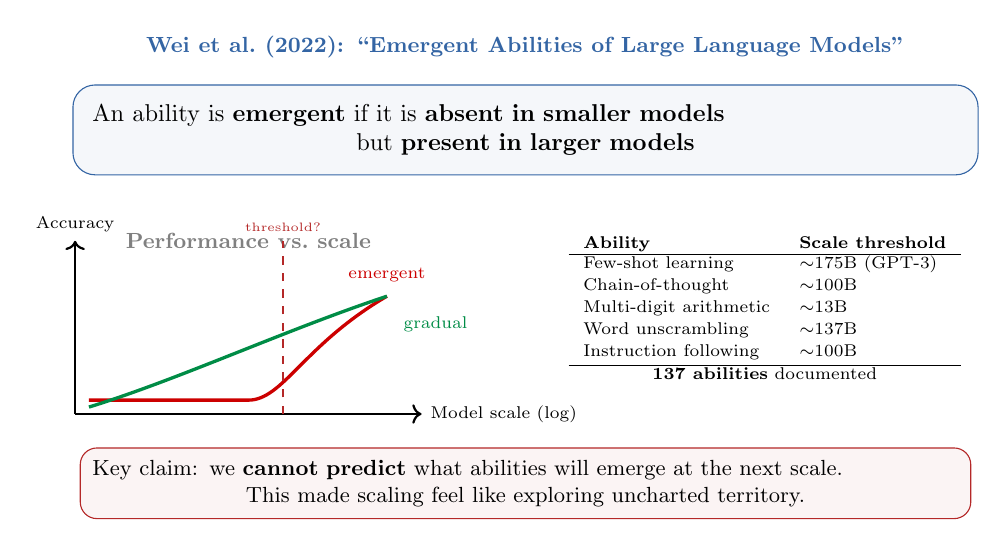
\begin{tikzpicture}[scale=0.88, transform shape]
  % Paper reference
  \node[font=\small\bfseries, text=popblue] at (0, 3.3) {Wei et al.\ (2022): ``Emergent Abilities of Large Language Models''};

  % Definition
  \node[draw=popblue, fill=popblue!5, rounded corners=8pt, text width=12.5cm, align=center, inner sep=8pt, font=\normalsize] at (0, 2.1) {
    An ability is \textbf{emergent} if it is \textbf{absent in smaller models}\newline
    but \textbf{present in larger models}
  };

  % The scaling plot sketch
  \node[font=\small\bfseries, text=gray] at (-4, 0.5) {Performance vs.\ scale};

  \draw[thick, ->] (-6.5, -2) -- (-1.5, -2) node[right, font=\scriptsize] {Model scale (log)};
  \draw[thick, ->] (-6.5, -2) -- (-6.5, 0.5) node[above, font=\scriptsize] {Accuracy};

  % Flat then jump (emergent)
  \draw[very thick, sampred] (-6.3, -1.8) -- (-4, -1.8) .. controls (-3.5, -1.8) and (-3.2, -1) .. (-2, -0.3);
  \node[font=\scriptsize, text=sampred] at (-2, 0) {emergent};

  % Gradual improvement (non-emergent)
  \draw[very thick, paramgreen] (-6.3, -1.9) .. controls (-5, -1.5) and (-3.5, -0.8) .. (-2, -0.3);
  \node[font=\scriptsize, text=paramgreen] at (-1.3, -0.7) {gradual};

  % Critical threshold
  \draw[dashed, warnred, thick] (-3.5, -2) -- (-3.5, 0.5);
  \node[font=\tiny, text=warnred] at (-3.5, 0.7) {threshold?};

  % Examples table
  \node at (3.5, -0.5) {
    {\scriptsize
    \begin{tabular}{l l}
      \textbf{Ability} & \textbf{Scale threshold} \\
      \hline
      Few-shot learning & $\sim$175B (GPT-3) \\[1pt]
      Chain-of-thought & $\sim$100B \\[1pt]
      Multi-digit arithmetic & $\sim$13B \\[1pt]
      Word unscrambling & $\sim$137B \\[1pt]
      Instruction following & $\sim$100B \\[1pt]
      \hline
      \multicolumn{2}{c}{\textbf{137 abilities} documented}
    \end{tabular}
    }
  };

  % Bottom note
  \node[draw=warnred, fill=warnred!5, rounded corners=6pt, text width=12.5cm, align=center, inner sep=5pt, font=\small] at (0, -3) {
    Key claim: we \textbf{cannot predict} what abilities will emerge at the next scale.\newline
    This made scaling feel like exploring uncharted territory.
  };
\end{tikzpicture}
\end{center}
\end{frame}

% ============================================================
% CHAIN-OF-THOUGHT AS EMERGENT
% ============================================================
\begin{frame}
\frametitle{Chain-of-thought: the poster child of emergence}
\vspace{-0.4cm}
\begin{center}
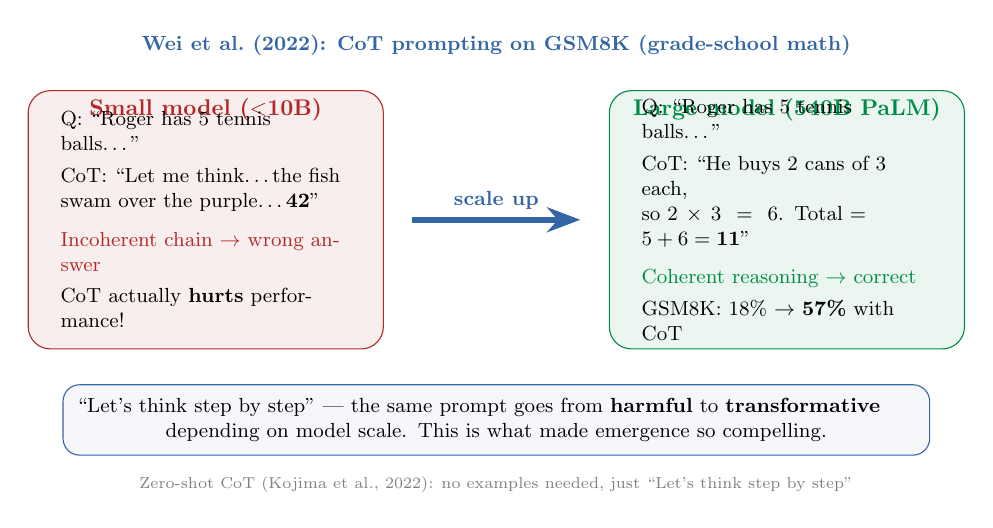
\begin{tikzpicture}[scale=0.82, transform shape]
  % The phenomenon
  \node[font=\small\bfseries, text=popblue] at (0, 3.5) {Wei et al.\ (2022): CoT prompting on GSM8K (grade-school math)};

  % Small model
  \node[draw=warnred, fill=warnred!8, rounded corners=8pt, minimum width=5.5cm, minimum height=4cm] at (-4.5, 0.8) {};
  \node[font=\normalsize\bfseries, text=warnred] at (-4.5, 2.5) {Small model ($<$10B)};

  \node[font=\small, text width=4.5cm, align=left] at (-4.5, 0.8) {
    Q: ``Roger has 5 tennis balls\ldots''\par\vspace{3pt}
    CoT: ``Let me think\ldots the fish\newline swam over the purple\ldots \textbf{42}''\par\vspace{6pt}
    \textcolor{warnred}{Incoherent chain $\to$ wrong answer}\par\vspace{3pt}
    CoT actually \textbf{hurts} performance!
  };

  % Large model
  \node[draw=paramgreen, fill=paramgreen!8, rounded corners=8pt, minimum width=5.5cm, minimum height=4cm] at (4.5, 0.8) {};
  \node[font=\normalsize\bfseries, text=paramgreen] at (4.5, 2.5) {Large model (540B PaLM)};

  \node[font=\small, text width=4.5cm, align=left] at (4.5, 0.8) {
    Q: ``Roger has 5 tennis balls\ldots''\par\vspace{3pt}
    CoT: ``He buys 2 cans of 3 each,\newline so $2\times 3=6$. Total = $5+6=\textbf{11}$''\par\vspace{6pt}
    \textcolor{paramgreen}{Coherent reasoning $\to$ correct}\par\vspace{3pt}
    GSM8K: 18\% $\to$ \textbf{57\%} with CoT
  };

  % Arrow between
  \draw[-Stealth, very thick, popblue, line width=2pt] (-1.3, 0.8) -- (1.3, 0.8)
    node[midway, above, font=\small\bfseries, text=popblue] {scale up};

  % Bottom insight
  \node[draw=popblue, fill=popblue!5, rounded corners=6pt, text width=13cm, align=center, inner sep=6pt, font=\small] at (0, -2.3) {
    ``Let's think step by step'' --- the same prompt goes from \textbf{harmful} to \textbf{transformative}\newline
    depending on model scale. This is what made emergence so compelling.
  };

  \node[font=\scriptsize, text=gray] at (0, -3.3) {
    Zero-shot CoT (Kojima et al., 2022): no examples needed, just ``Let's think step by step''
  };
\end{tikzpicture}
\end{center}
\end{frame}

% ============================================================
% THE MIRAGE CRITIQUE
% ============================================================
\begin{frame}
\frametitle{Are emergent abilities a mirage?}
\vspace{-0.3cm}
\begin{center}
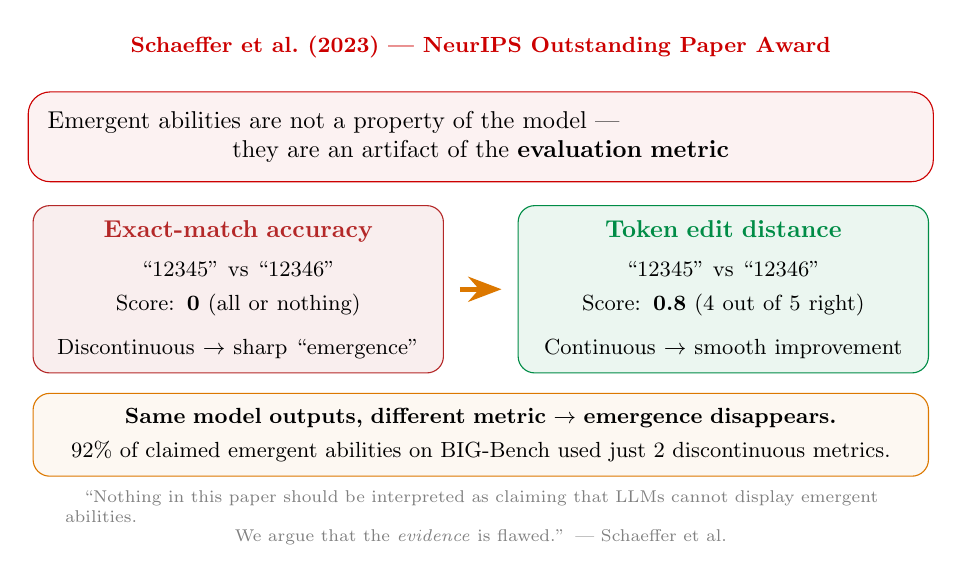
\begin{tikzpicture}[scale=0.88, transform shape]
  % Paper reference
  \node[font=\small\bfseries, text=sampred] at (0, 3.3) {Schaeffer et al.\ (2023) --- NeurIPS Outstanding Paper Award};

  % Core claim
  \node[draw=sampred, fill=sampred!5, rounded corners=8pt, text width=12.5cm, align=center, inner sep=8pt, font=\normalsize] at (0, 2) {
    Emergent abilities are not a property of the model ---\newline
    they are an artifact of the \textbf{evaluation metric}
  };

  % Two metrics side by side
  \node[draw=warnred, fill=warnred!8, rounded corners=6pt, text width=5.5cm, align=center, inner sep=6pt] at (-3.5, -0.2) {
    \textbf{\textcolor{warnred}{Exact-match accuracy}}\par\vspace{4pt}
    {\small ``12345'' vs ``12346''}\par\vspace{2pt}
    {\small Score: \textbf{0} (all or nothing)}\par\vspace{6pt}
    {\small Discontinuous $\to$ sharp ``emergence''}
  };

  \node[draw=paramgreen, fill=paramgreen!8, rounded corners=6pt, text width=5.5cm, align=center, inner sep=6pt] at (3.5, -0.2) {
    \textbf{\textcolor{paramgreen}{Token edit distance}}\par\vspace{4pt}
    {\small ``12345'' vs ``12346''}\par\vspace{2pt}
    {\small Score: \textbf{0.8} (4 out of 5 right)}\par\vspace{6pt}
    {\small Continuous $\to$ smooth improvement}
  };

  \draw[-Stealth, very thick, orange1, line width=2pt] (-0.3, -0.2) -- (0.3, -0.2);

  % Key finding
  \node[draw=orange1, fill=orange1!5, rounded corners=6pt, text width=12.5cm, align=center, inner sep=6pt, font=\small] at (0, -2.3) {
    \textbf{Same model outputs, different metric $\to$ emergence disappears.}\par\vspace{3pt}
    92\% of claimed emergent abilities on BIG-Bench used just 2 discontinuous metrics.
  };

  % Bottom note
  \node[font=\scriptsize, text=gray, text width=12cm, align=center] at (0, -3.5) {
    ``Nothing in this paper should be interpreted as claiming that LLMs cannot display emergent abilities.\newline
    We argue that the \textit{evidence} is flawed.'' --- Schaeffer et al.
  };
\end{tikzpicture}
\end{center}
\end{frame}

% ============================================================
% THE METRIC ILLUSION — VISUALIZED
% ============================================================
\begin{frame}
\frametitle{The metric illusion}
\vspace{-0.4cm}
\begin{center}
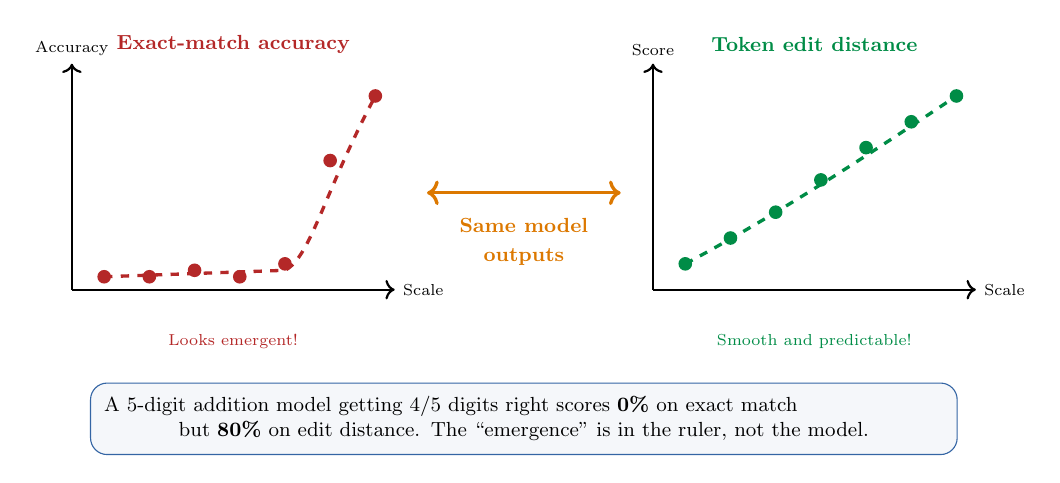
\begin{tikzpicture}[scale=0.82, transform shape]
  % Left plot: discontinuous metric
  \node[font=\small\bfseries, text=warnred] at (-4.5, 3.3) {Exact-match accuracy};

  \draw[thick, ->] (-7, -0.5) -- (-2, -0.5) node[right, font=\scriptsize] {Scale};
  \draw[thick, ->] (-7, -0.5) -- (-7, 3) node[above, font=\scriptsize] {Accuracy};

  % Data points - flat then jump
  \fill[warnred] (-6.5, -0.3) circle (3pt);
  \fill[warnred] (-5.8, -0.3) circle (3pt);
  \fill[warnred] (-5.1, -0.2) circle (3pt);
  \fill[warnred] (-4.4, -0.3) circle (3pt);
  \fill[warnred] (-3.7, -0.1) circle (3pt);
  \fill[warnred] (-3.0, 1.5) circle (3pt);
  \fill[warnred] (-2.3, 2.5) circle (3pt);

  % Fit line
  \draw[very thick, warnred, dashed] (-6.5, -0.3) -- (-3.7, -0.2) .. controls (-3.3, 0) and (-3.1, 1) .. (-2.3, 2.5);

  \node[font=\scriptsize, text=warnred] at (-4.5, -1.3) {Looks emergent!};

  % Right plot: continuous metric
  \node[font=\small\bfseries, text=paramgreen] at (4.5, 3.3) {Token edit distance};

  \draw[thick, ->] (2, -0.5) -- (7, -0.5) node[right, font=\scriptsize] {Scale};
  \draw[thick, ->] (2, -0.5) -- (2, 3) node[above, font=\scriptsize] {Score};

  % Data points - smooth improvement
  \fill[paramgreen] (2.5, -0.1) circle (3pt);
  \fill[paramgreen] (3.2, 0.3) circle (3pt);
  \fill[paramgreen] (3.9, 0.7) circle (3pt);
  \fill[paramgreen] (4.6, 1.2) circle (3pt);
  \fill[paramgreen] (5.3, 1.7) circle (3pt);
  \fill[paramgreen] (6.0, 2.1) circle (3pt);
  \fill[paramgreen] (6.7, 2.5) circle (3pt);

  % Fit line
  \draw[very thick, paramgreen, dashed] (2.5, -0.1) .. controls (4, 0.7) and (5.5, 1.7) .. (6.7, 2.5);

  \node[font=\scriptsize, text=paramgreen] at (4.5, -1.3) {Smooth and predictable!};

  % Center annotation
  \draw[very thick, orange1, <->] (-1.5, 1) -- (1.5, 1);
  \node[font=\small\bfseries, text=orange1] at (0, 0.5) {Same model};
  \node[font=\small\bfseries, text=orange1] at (0, 0.0) {outputs};

  % Key insight
  \node[draw=popblue, fill=popblue!5, rounded corners=6pt, text width=13cm, align=center, inner sep=6pt, font=\small] at (0, -2.5) {
    A 5-digit addition model getting 4/5 digits right scores \textbf{0\%} on exact match\newline
    but \textbf{80\%} on edit distance. The ``emergence'' is in the ruler, not the model.
  };
\end{tikzpicture}
\end{center}
\end{frame}

% ============================================================
% THE AND-GATE ARGUMENT
% ============================================================
\begin{frame}
\frametitle{The AND-gate: why some emergence might be real}
\vspace{-0.3cm}
\begin{center}
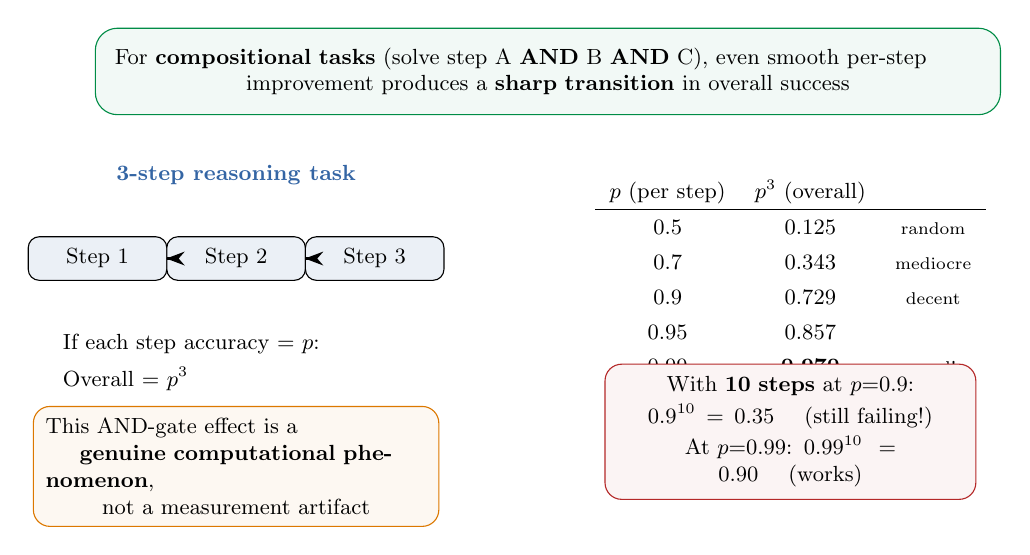
\begin{tikzpicture}[scale=0.88, transform shape]
  % The argument
  \node[draw=paramgreen, fill=paramgreen!5, rounded corners=8pt, text width=12.5cm, align=center, inner sep=8pt, font=\small] at (0, 3) {
    For \textbf{compositional tasks} (solve step A \textbf{AND} B \textbf{AND} C), even smooth per-step\newline
    improvement produces a \textbf{sharp transition} in overall success
  };

  % Math example
  \node[font=\small\bfseries, text=popblue] at (-4.5, 1.5) {3-step reasoning task};

  % Three steps as gates
  \node[draw, rounded corners=4pt, fill=popblue!10, minimum width=2cm, font=\small, inner sep=5pt] (s1) at (-6.5, 0.3) {Step 1};
  \node[draw, rounded corners=4pt, fill=popblue!10, minimum width=2cm, font=\small, inner sep=5pt] (s2) at (-4.5, 0.3) {Step 2};
  \node[draw, rounded corners=4pt, fill=popblue!10, minimum width=2cm, font=\small, inner sep=5pt] (s3) at (-2.5, 0.3) {Step 3};

  \draw[-Stealth, thick] (s1) -- (s2);
  \draw[-Stealth, thick] (s2) -- (s3);

  % Probability calculation
  \node[font=\small, text width=5cm, align=left] at (-4.5, -1.2) {
    If each step accuracy = $p$:\par\vspace{4pt}
    Overall = $p^3$
  };

  % Table
  \node at (3.5, 0) {
    {\small
    \renewcommand{\arraystretch}{1.3}
    \begin{tabular}{c c c}
      $p$ (per step) & $p^3$ (overall) & \\
      \hline
      0.5 & 0.125 & {\scriptsize random} \\
      0.7 & 0.343 & {\scriptsize mediocre} \\
      0.9 & 0.729 & {\scriptsize decent} \\
      0.95 & 0.857 & \\
      0.99 & \textbf{0.970} & {\scriptsize good!} \\
    \end{tabular}
    }
  };

  % Longer chains
  \node[draw=warnred, fill=warnred!5, rounded corners=6pt, text width=5cm, align=center, inner sep=5pt, font=\small] at (3.5, -2.2) {
    With \textbf{10 steps} at $p{=}0.9$:\par\vspace{2pt}
    $0.9^{10} = 0.35$ \quad (still failing!)\par\vspace{2pt}
    At $p{=}0.99$: $0.99^{10} = 0.90$ \quad (works)
  };

  % Key insight
  \node[draw=orange1, fill=orange1!5, rounded corners=6pt, text width=5.5cm, align=center, inner sep=5pt, font=\small] at (-4.5, -2.7) {
    This AND-gate effect is a\newline
    \textbf{genuine computational phenomenon},\newline
    not a measurement artifact
  };
\end{tikzpicture}
\end{center}
\end{frame}

% ============================================================
% WHERE THE DEBATE STANDS
% ============================================================
\begin{frame}
\frametitle{Where the debate stands today}
\vspace{-0.3cm}
\begin{center}
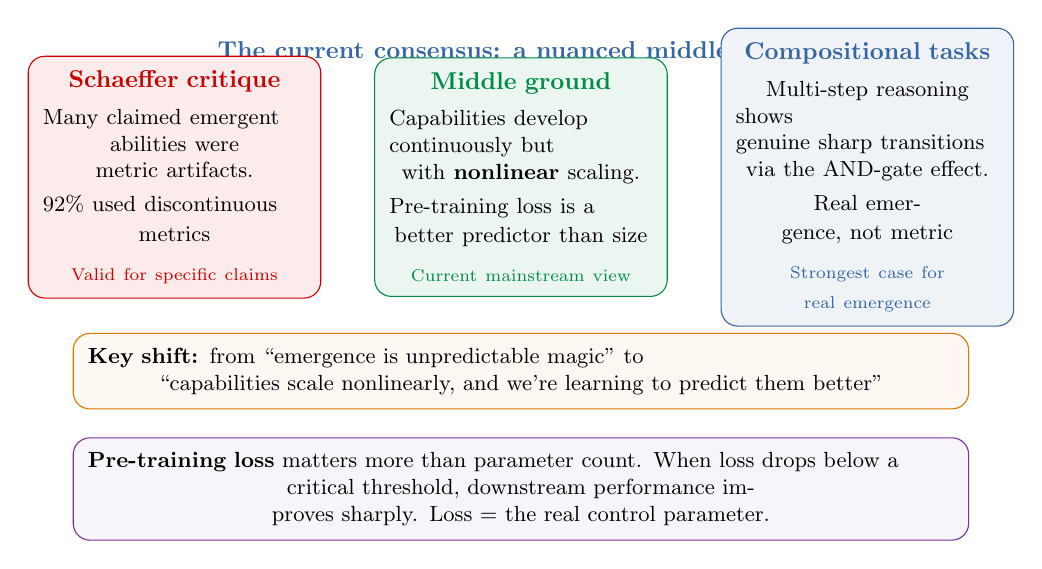
\begin{tikzpicture}[scale=0.88, transform shape]
  % Spectrum
  \node[font=\normalsize\bfseries, text=popblue] at (0, 3.3) {The current consensus: a nuanced middle ground};

  % Three positions
  \node[draw=sampred, fill=sampred!8, rounded corners=6pt, text width=3.8cm, align=center, inner sep=6pt] at (-5, 1.5) {
    \textbf{\textcolor{sampred}{Schaeffer critique}}\par\vspace{4pt}
    {\small Many claimed emergent\newline abilities were metric artifacts.\par\vspace{2pt}
    92\% used discontinuous\newline metrics}\par\vspace{4pt}
    {\scriptsize\textcolor{sampred}{Valid for specific claims}}
  };

  \node[draw=paramgreen, fill=paramgreen!8, rounded corners=6pt, text width=3.8cm, align=center, inner sep=6pt] at (0, 1.5) {
    \textbf{\textcolor{paramgreen}{Middle ground}}\par\vspace{4pt}
    {\small Capabilities develop\newline continuously but\newline with \textbf{nonlinear} scaling.\par\vspace{2pt}
    Pre-training loss is a\newline better predictor than size}\par\vspace{4pt}
    {\scriptsize\textcolor{paramgreen}{Current mainstream view}}
  };

  \node[draw=popblue, fill=popblue!8, rounded corners=6pt, text width=3.8cm, align=center, inner sep=6pt] at (5, 1.5) {
    \textbf{\textcolor{popblue}{Compositional tasks}}\par\vspace{4pt}
    {\small Multi-step reasoning shows\newline genuine sharp transitions\newline via the AND-gate effect.\par\vspace{2pt}
    Real emergence, not metric}\par\vspace{4pt}
    {\scriptsize\textcolor{popblue}{Strongest case for real emergence}}
  };

  % Key shift
  \node[draw=orange1, fill=orange1!5, rounded corners=6pt, text width=12.5cm, align=center, inner sep=6pt, font=\small] at (0, -1.3) {
    \textbf{Key shift:} from ``emergence is unpredictable magic'' to\newline
    ``capabilities scale nonlinearly, and we're learning to predict them better''
  };

  % Pre-training loss insight
  \node[draw=violet1, fill=violet1!5, rounded corners=6pt, text width=12.5cm, align=center, inner sep=6pt, font=\small] at (0, -3) {
    \textbf{Pre-training loss} matters more than parameter count. When loss drops below a\newline
    critical threshold, downstream performance improves sharply. Loss $=$ the real control parameter.
  };
\end{tikzpicture}
\end{center}
\end{frame}

% ============================================================
% GROKKING
% ============================================================
\begin{frame}
\frametitle{Grokking: delayed generalization}
\vspace{-0.4cm}
\begin{center}
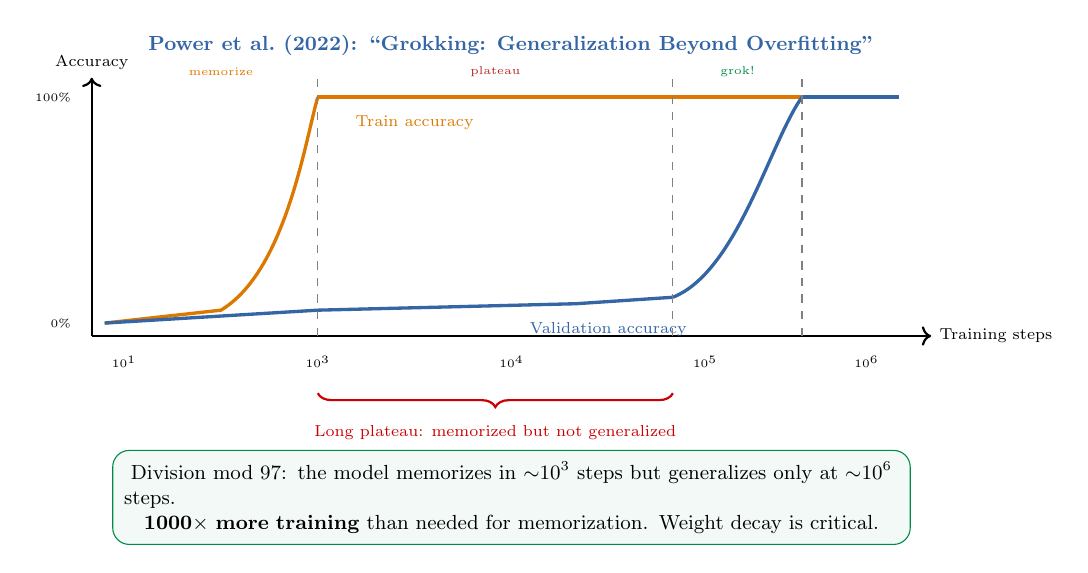
\begin{tikzpicture}[scale=0.82, transform shape]
  % Paper reference
  \node[font=\small\bfseries, text=popblue] at (0, 3.5) {Power et al.\ (2022): ``Grokking: Generalization Beyond Overfitting''};

  % Training plot
  \draw[thick, ->] (-6.5, -1) -- (6.5, -1) node[right, font=\scriptsize] {Training steps};
  \draw[thick, ->] (-6.5, -1) -- (-6.5, 3) node[above, font=\scriptsize] {Accuracy};

  % Axis labels
  \node[font=\tiny, anchor=east] at (-6.7, -0.8) {0\%};
  \node[font=\tiny, anchor=east] at (-6.7, 2.7) {100\%};
  \node[font=\tiny] at (-6, -1.4) {$10^1$};
  \node[font=\tiny] at (-3, -1.4) {$10^3$};
  \node[font=\tiny] at (0, -1.4) {$10^4$};
  \node[font=\tiny] at (3, -1.4) {$10^5$};
  \node[font=\tiny] at (5.5, -1.4) {$10^6$};

  % Training accuracy (orange - fast)
  \draw[very thick, orange1] (-6.3, -0.8) -- (-4.5, -0.6) .. controls (-3.5, 0) and (-3.2, 2) .. (-3, 2.7);
  \draw[very thick, orange1] (-3, 2.7) -- (6, 2.7);
  \node[font=\scriptsize, text=orange1] at (-1.5, 2.3) {Train accuracy};

  % Validation accuracy (blue - delayed)
  \draw[very thick, popblue] (-6.3, -0.8) -- (-3, -0.6) -- (1, -0.5) -- (2.5, -0.4);
  \draw[very thick, popblue] (2.5, -0.4) .. controls (3.5, 0) and (4, 2) .. (4.5, 2.7);
  \draw[very thick, popblue] (4.5, 2.7) -- (6, 2.7);
  \node[font=\scriptsize, text=popblue] at (1.5, -0.9) {Validation accuracy};

  % Annotations
  \draw[decorate, decoration={brace, amplitude=5pt, raise=2pt, mirror}, thick, sampred] (-3, -1.8) -- (2.5, -1.8);
  \node[font=\scriptsize, text=sampred] at (-0.25, -2.5) {Long plateau: memorized but not generalized};

  % Phase labels
  \draw[dashed, gray] (-3, -1) -- (-3, 3);
  \draw[dashed, gray] (2.5, -1) -- (2.5, 3);
  \draw[dashed, gray] (4.5, -1) -- (4.5, 3);

  \node[font=\tiny, text=orange1] at (-4.5, 3.1) {memorize};
  \node[font=\tiny, text=warnred] at (-0.25, 3.1) {plateau};
  \node[font=\tiny, text=paramgreen] at (3.5, 3.1) {grok!};

  % Key insight
  \node[draw=paramgreen, fill=paramgreen!5, rounded corners=6pt, text width=12cm, align=center, inner sep=5pt, font=\small] at (0, -3.5) {
    Division mod 97: the model memorizes in $\sim$10$^3$ steps but generalizes only at $\sim$10$^6$ steps.\newline
    \textbf{1000$\times$ more training} than needed for memorization. Weight decay is critical.
  };
\end{tikzpicture}
\end{center}
\end{frame}

% ============================================================
% GROKKING AND EMERGENCE
% ============================================================
\begin{frame}
\frametitle{Grokking and emergence: the common pattern}
\vspace{-0.3cm}
\begin{center}
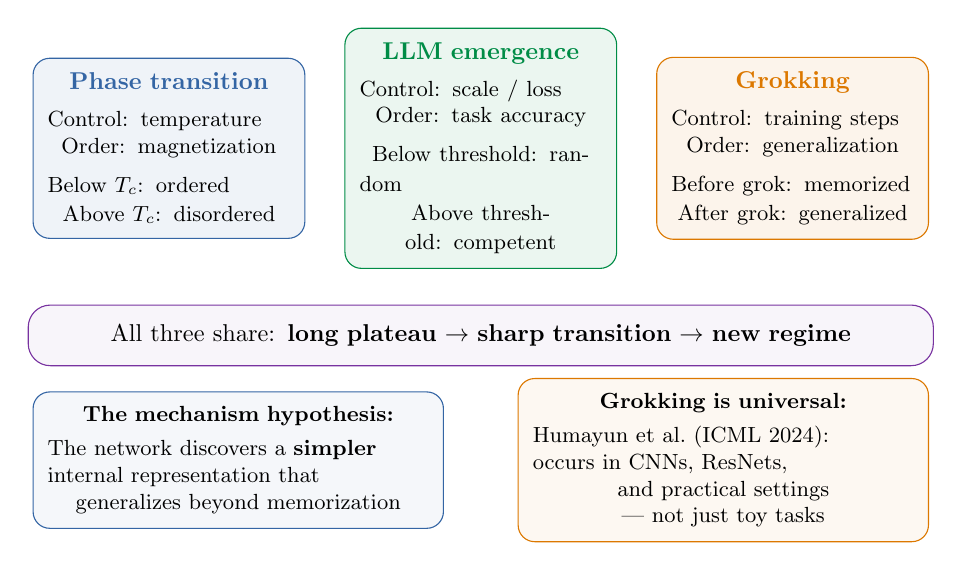
\begin{tikzpicture}[scale=0.88, transform shape]
  % Three phenomena side by side
  \node[draw=popblue, fill=popblue!8, rounded corners=6pt, text width=3.5cm, align=center, inner sep=6pt] at (-4.5, 2) {
    \textbf{\textcolor{popblue}{Phase transition}}\par\vspace{4pt}
    {\small Control: temperature\newline Order: magnetization\par\vspace{4pt}
    Below $T_c$: ordered\newline Above $T_c$: disordered}
  };

  \node[draw=paramgreen, fill=paramgreen!8, rounded corners=6pt, text width=3.5cm, align=center, inner sep=6pt] at (0, 2) {
    \textbf{\textcolor{paramgreen}{LLM emergence}}\par\vspace{4pt}
    {\small Control: scale / loss\newline Order: task accuracy\par\vspace{4pt}
    Below threshold: random\newline Above threshold: competent}
  };

  \node[draw=orange1, fill=orange1!8, rounded corners=6pt, text width=3.5cm, align=center, inner sep=6pt] at (4.5, 2) {
    \textbf{\textcolor{orange1}{Grokking}}\par\vspace{4pt}
    {\small Control: training steps\newline Order: generalization\par\vspace{4pt}
    Before grok: memorized\newline After grok: generalized}
  };

  % Common pattern
  \node[draw=violet1, fill=violet1!5, rounded corners=8pt, text width=12.5cm, align=center, inner sep=8pt, font=\normalsize] at (0, -0.7) {
    All three share: \textbf{long plateau} $\to$ \textbf{sharp transition} $\to$ \textbf{new regime}
  };

  % Deeper connection
  \node[draw=popblue, fill=popblue!5, rounded corners=6pt, text width=5.5cm, align=center, inner sep=6pt, font=\small] at (-3.5, -2.5) {
    \textbf{The mechanism hypothesis:}\par\vspace{3pt}
    The network discovers a \textbf{simpler}\newline internal representation that\newline generalizes beyond memorization
  };

  \node[draw=orange1, fill=orange1!5, rounded corners=6pt, text width=5.5cm, align=center, inner sep=6pt, font=\small] at (3.5, -2.5) {
    \textbf{Grokking is universal:}\par\vspace{3pt}
    Humayun et al.\ (ICML 2024):\newline
    occurs in CNNs, ResNets,\newline
    and practical settings --- not just toy tasks
  };
\end{tikzpicture}
\end{center}
\end{frame}

% ============================================================
% WEAK VS STRONG EMERGENCE
% ============================================================
\begin{frame}
\frametitle{Weak vs.\ strong emergence}
\vspace{-0.3cm}
\begin{center}
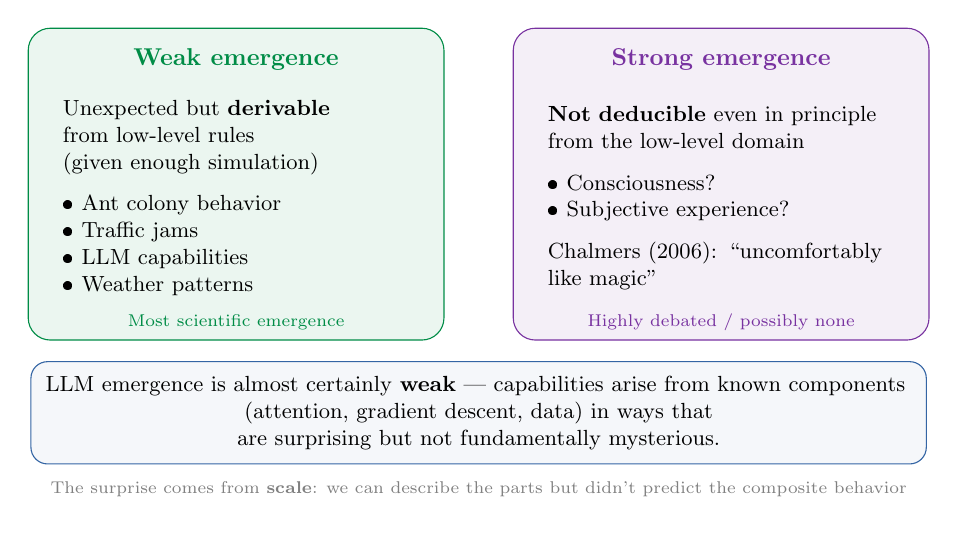
\begin{tikzpicture}[scale=0.88, transform shape]
  % Two columns
  \node[draw=paramgreen, fill=paramgreen!8, rounded corners=8pt, minimum width=6cm, minimum height=4.5cm] at (-3.5, 1) {};
  \node[font=\normalsize\bfseries, text=paramgreen] at (-3.5, 2.8) {Weak emergence};

  \node[font=\small, text width=5cm, align=left] at (-3.5, 0.8) {
    Unexpected but \textbf{derivable}\newline from low-level rules\newline (given enough simulation)\par\vspace{6pt}
    \textbullet\ Ant colony behavior\newline
    \textbullet\ Traffic jams\newline
    \textbullet\ LLM capabilities\newline
    \textbullet\ Weather patterns
  };
  \node[font=\scriptsize, text=paramgreen] at (-3.5, -1) {Most scientific emergence};

  \node[draw=violet1, fill=violet1!8, rounded corners=8pt, minimum width=6cm, minimum height=4.5cm] at (3.5, 1) {};
  \node[font=\normalsize\bfseries, text=violet1] at (3.5, 2.8) {Strong emergence};

  \node[font=\small, text width=5cm, align=left] at (3.5, 0.8) {
    \textbf{Not deducible} even in principle\newline from the low-level domain\par\vspace{6pt}
    \textbullet\ Consciousness?\newline
    \textbullet\ Subjective experience?\par\vspace{6pt}
    Chalmers (2006): ``uncomfortably\newline like magic''
  };
  \node[font=\scriptsize, text=violet1] at (3.5, -1) {Highly debated / possibly none};

  % Where do LLMs fall?
  \node[draw=popblue, fill=popblue!5, rounded corners=6pt, text width=12.5cm, align=center, inner sep=6pt, font=\small] at (0, -2.3) {
    LLM emergence is almost certainly \textbf{weak} --- capabilities arise from known components\newline (attention, gradient descent, data) in ways that are surprising but not fundamentally mysterious.
  };

  \node[font=\scriptsize, text=gray] at (0, -3.4) {
    The surprise comes from \textbf{scale}: we can describe the parts but didn't predict the composite behavior
  };
\end{tikzpicture}
\end{center}
\end{frame}

% ============================================================
% IMPLICATIONS
% ============================================================
\begin{frame}
\frametitle{Why emergence matters for AI}
\vspace{-0.3cm}
\begin{center}
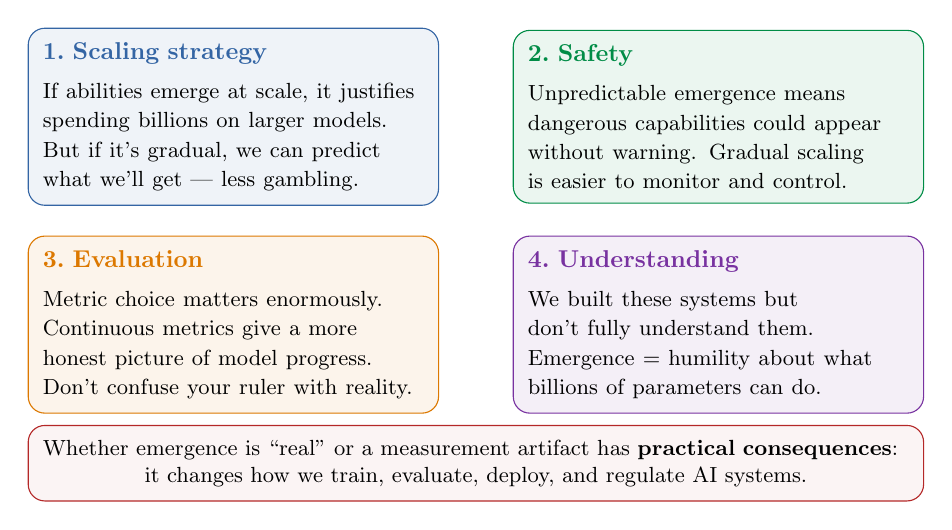
\begin{tikzpicture}[scale=0.88, transform shape]
  % Four implication boxes
  \node[draw=popblue, fill=popblue!8, rounded corners=6pt, text width=5.5cm, align=left, inner sep=6pt] at (-3.5, 2) {
    \textbf{\textcolor{popblue}{1.\ Scaling strategy}}\par\vspace{4pt}
    {\small If abilities emerge at scale, it justifies\newline spending billions on larger models.\newline But if it's gradual, we can predict\newline what we'll get --- less gambling.}
  };

  \node[draw=paramgreen, fill=paramgreen!8, rounded corners=6pt, text width=5.5cm, align=left, inner sep=6pt] at (3.5, 2) {
    \textbf{\textcolor{paramgreen}{2.\ Safety}}\par\vspace{4pt}
    {\small Unpredictable emergence means\newline dangerous capabilities could appear\newline without warning. Gradual scaling\newline is easier to monitor and control.}
  };

  \node[draw=orange1, fill=orange1!8, rounded corners=6pt, text width=5.5cm, align=left, inner sep=6pt] at (-3.5, -1) {
    \textbf{\textcolor{orange1}{3.\ Evaluation}}\par\vspace{4pt}
    {\small Metric choice matters enormously.\newline Continuous metrics give a more\newline honest picture of model progress.\newline Don't confuse your ruler with reality.}
  };

  \node[draw=violet1, fill=violet1!8, rounded corners=6pt, text width=5.5cm, align=left, inner sep=6pt] at (3.5, -1) {
    \textbf{\textcolor{violet1}{4.\ Understanding}}\par\vspace{4pt}
    {\small We built these systems but\newline don't fully understand them.\newline Emergence = humility about what\newline billions of parameters can do.}
  };

  % Bottom
  \node[draw=warnred, fill=warnred!5, rounded corners=6pt, text width=12.5cm, align=center, inner sep=6pt, font=\small] at (0, -3) {
    Whether emergence is ``real'' or a measurement artifact has \textbf{practical consequences}:\newline
    it changes how we train, evaluate, deploy, and regulate AI systems.
  };
\end{tikzpicture}
\end{center}
\end{frame}

% ============================================================
% FURTHER READING
% ============================================================
\begin{frame}
\frametitle{Further reading}
\vspace{-0.3cm}
\begin{center}
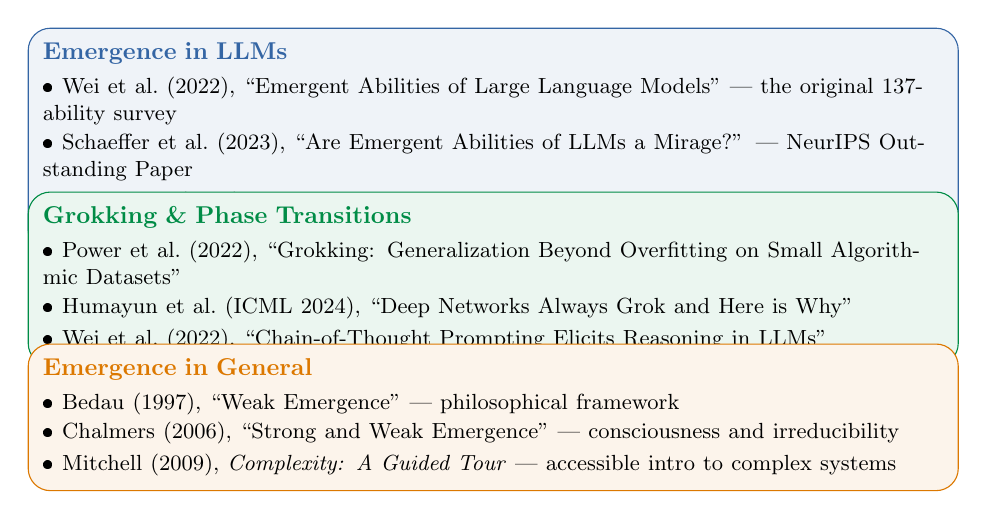
\begin{tikzpicture}[scale=0.88, transform shape]
  \node[draw=popblue, fill=popblue!8, rounded corners=8pt, text width=13cm, align=left, inner sep=6pt] at (0, 2.5) {
    \textbf{\textcolor{popblue}{Emergence in LLMs}}\par\vspace{3pt}
    {\small
    \textbullet~Wei et al.\ (2022), ``Emergent Abilities of Large Language Models'' --- the original 137-ability survey\par\vspace{1pt}
    \textbullet~Schaeffer et al.\ (2023), ``Are Emergent Abilities of LLMs a Mirage?'' --- NeurIPS Outstanding Paper\par\vspace{1pt}
    \textbullet~Berti et al.\ (2025), ``Emergent Abilities in LLMs: A Survey'' --- most recent comprehensive review
    }
  };

  \node[draw=paramgreen, fill=paramgreen!8, rounded corners=8pt, text width=13cm, align=left, inner sep=6pt] at (0, 0.5) {
    \textbf{\textcolor{paramgreen}{Grokking \& Phase Transitions}}\par\vspace{3pt}
    {\small
    \textbullet~Power et al.\ (2022), ``Grokking: Generalization Beyond Overfitting on Small Algorithmic Datasets''\par\vspace{1pt}
    \textbullet~Humayun et al.\ (ICML 2024), ``Deep Networks Always Grok and Here is Why''\par\vspace{1pt}
    \textbullet~Wei et al.\ (2022), ``Chain-of-Thought Prompting Elicits Reasoning in LLMs''
    }
  };

  \node[draw=orange1, fill=orange1!8, rounded corners=8pt, text width=13cm, align=left, inner sep=6pt] at (0, -1.5) {
    \textbf{\textcolor{orange1}{Emergence in General}}\par\vspace{3pt}
    {\small
    \textbullet~Bedau (1997), ``Weak Emergence'' --- philosophical framework\par\vspace{1pt}
    \textbullet~Chalmers (2006), ``Strong and Weak Emergence'' --- consciousness and irreducibility\par\vspace{1pt}
    \textbullet~Mitchell (2009), \emph{Complexity: A Guided Tour} --- accessible intro to complex systems
    }
  };
\end{tikzpicture}
\end{center}
\end{frame}

% ============================================================
% QUESTIONS
% ============================================================
\begin{frame}
\begin{center}
\vspace{2cm}
{\Huge \textcolor{popblue}{Questions?}}

\vspace{1cm}
\end{center}
\end{frame}

\end{document}
